%-------------------------------------------------------------------------------
% Arquivo: 		memorial.tex
% Autor:			Ivan Ramos Pagnossin
% Descrição:	Memorial escrito para o concurso de admissão de docente no IFUSP
%-------------------------------------------------------------------------------
\documentclass[a4paper,12pt,twoside]{scrartcl}					% Sub-classe koma-script

	%
	% Pacotes necessários.
	%
	\usepackage[brazil]{babel}								% Idioma português
	\usepackage[utf8]{inputenc}							% Caracteres acentuados
	\usepackage[T1]{fontenc}								% Fontes de 16 bits
	\usepackage{fouriernc}
	\usepackage{xcolor}										% Cores
	\usepackage[a4paper, top=3cm, left=3cm, right=2cm, bottom=2cm, includefoot]{geometry}						% Formatação de página
	\usepackage{indentfirst}								% Indentação do primeiro parágrafo de cada seção
	\usepackage{setspace}									% Espaçamento entre-linhas
	\usepackage[squaren,binary]{SIunits}				% Sistema internacional de unidades
	\usepackage{amsmath}										% Environments e comandos da American Mathematical Society	
	\usepackage{paralist}									% Environment "compactitem"
  \usepackage{url}
  \usepackage{fancyhdr}
  \usepackage[symbol,norule,flushmargin]{footmisc}
    \usepackage[colorlinks=true,linkcolor=blue,urlcolor=blue]{hyperref}
      \usepackage{graphicx}

	%
	% Definições úteis.
	%
	\newcommand\foreign[1]{\textnormal{#1}}
	\newcommand\edital[1]{\textnormal{#1}}%\textcolor{green!30!black}{#1}}
	\newcommand\profa{Prof\rlap.\textordfeminine}
	\newcommand\etc{\foreign{etc}}
	\newcommand\dra{Dr\rlap.\textordfeminine}
	\newcommand\ie{\foreign{ie}}

	% Insere minhas definições de formato (REORGANIZAR).
	\input{myPortuges.ldf}

	% Impede que o texto seja uniformemente distribuído na vertical.
	\raggedbottom

	% Espaço entre-linhas: 30% maior que o normal.
	\setstretch{1.3}

	% Configuração manual da divisão silábica de algumas palavras.
	\hyphenation{}

	% Configuração dos cabeçalhos e rodapés
	\pagestyle{fancy}
	\fancyhead{}
	\fancyhead[LE]{I. R. Pagnossin}
	\fancyhead[RE]{}
	\fancyhead[LO]{}
	\fancyhead[RO]{{\footnotesize Memorial circunstanciado}}
	\fancyfoot{}
	\fancyfoot[LE,RO]{\thepage}
	\fancyfoot[RE,LO]{}
	\renewcommand\footrulewidth{0.4pt}
	
	% Configuração das notas de rodapé
	\setfnsymbol{lamport}

	% Configuração da capa
	\title{Memorial circunstanciado}
	\author{Ivan Ramos Pagnossin}
	
	\hyphenation{E-le-trô-ni-ca E-le-tro-pi-e-zo dou-to-ra-do pe-da-gó-gi-co do-mi-nar e-xa-me gra-du-a-ção he-te-ro-es-tru-tu-ras re-gis-tra-do a-pre-sen-ta-ção}
	
%-------------------------------------------------------------------------------
%-------------------------------------------------------------------------------
%	Aqui começa o documento propriamente dito.
%-------------------------------------------------------------------------------
%-------------------------------------------------------------------------------


\begin{document}

	\maketitle
	%\tableofcontents
	%\pagenumbering{roman}

	% Prefácio
	%\pagebreak
	%\pagenumbering{arabic}
	%\setcounter{page}{1}
	
	\chapter{Apresenta��o}

Caro Professor, n�o vejo maneira mais honesta de me apresentar do que permitir que algu�m o fa�a por mim. Por isso, gostaria de come�ar este memorial com um depoimento dado pelo Prof. Dr. Ewout ter Haar, com quem tenho o prazer de trabalhar desde dezembro de 2007, em meu perfil no LinkedIn (\url{linkedin.com}). Em suas palavras: (sic)

\begin{quotation}

{\itshape Ivan trabalhou por aproximadamente 2 anos no nosso grupo na �rea de tecnologia educacional. O n�vel e quantidade de conhecimento e habilidade agregado ao grupo foi muito alto. Neste per�odo executava os projetos sugeridos com extrema efici�ncia e originalidade. Mas trouxe tamb�m novos projetos e ideias ao grupo. As discuss�es sobre assuntos t�cnicos foram de alta intensidade e proveitoso para todos. 

O Ivan se tornou especialista em ensino a dist�ncia, anima��es interativas e material did�tico digital de uma forma geral. Entretanto, mais importante do que qualquer habilidade em particular, se mostrou capaz de adquirir novas habilidades e dominar novas tecnologias muito r�pido}

\begin{flushright}
Ewout ter Haar,\\8 de maio de 2009
\end{flushright}

\end{quotation}

Nas p�ginas seguintes, apresentarei minha trajet�ria educacional e profissional, destacando as principais atividades que desenvolvi e mostrando como elas me trouxeram at� aqui. Este documento tamb�m revela, no cap�tulo~\ref{cap:projeto-pesquisa}, o projeto de pesquisa que pretendo desenvolver como docente do IF. E o ap�ndice \ref{cap:resumo} cont�m um resumo das produ��es mais relevantes da minha carreira.

Para registro, este material foi escrito com vistas ao concurso de t�tulos e provas para o provimento de um cargo de Professor Doutor junto ao Departamento de F�sica Experimental do Instituto de F�sica (IF) da Universidade de S�o Paulo (USP), edital IF n�mero 19/2011, de 19 de mar�o de 2011. Ao longo do texto, as palavras destacadas \edital{desta maneira} foram apresentadas no edital como parte da qualifica��o necess�ria para concorrer ao cargo.


	\chapter{Formação acadêmica}

Minha formação acadêmica sempre foi voltada para o estudo da Física Básica e Aplicada, particularmente na área de materiais semicondutores e de fenômenos de transporte eletrônico. No entanto, ela sofreu grande influência da minha formação profissional (capítulo~\ref{cap:formacao-profissional}) --- bem como a influenciou ---, especialmente no que concerne o desenvolvimento de \foreign{software}.

\section{Graduação e iniciação científica}
\label{sec:graduacao}

Minha formação acadêmica começou em fevereiro de 1997, quando fui aprovado no exame vestibular da USP para o curso de Bacharelado em Física, no \foreign{campus} da capital. A escolha pela Física foi moldada, anos antes, pelo contato com circuitos eletrônicos, no ensino médio profissionalizante (seção~\ref{sec:liceu}), bem como por uma paixão ainda mais antiga: a aviação. Já a opção pelo bacharelado foi feita pelo desejo de aprender \emph{profundamente} fenômenos físicos e técnicas matemáticas, em muito alimentado pelo aprendizado autodidata de cálculo diferencial e integral, ainda no ensino médio.

Na verdade, o fato de eu já conhecer o cálculo diferencial e integral ao começar a graduação ajudou-me enormemente, permitindo-me aproveitar melhor os conceitos e técnicas ensinados, bem como ir além deles, em todas as disciplinas cursadas. De fato, em oposição ao que ocorreu durante o ensino médio (veja a seção \ref{sec:liceu}), eu me destaquei em praticamente todas as disciplinas, chegando a atingir médias como 9,5 em disciplinas como Cálculo, Álgebra Linear, Física Atômica e Molecular, entre outras.

O ensino médio profissionalizante teve outra clara e positiva influência na minha graduação: logo na primeira semana consegui uma bolsa de iniciação científica do CNPq no Laboratório de Física de Plasmas, orientado pelo Prof. Dr. Ivan Cunha Nascimento, e em muito auxiliado pelo funcionário Juan Iraburu Elizondo. A proposta era a de estudar a chamada curva de \foreign{breakdown}, que caracterizava a formação de plasma no Tokamak. Os resultados deste trabalho foram apresentados no Simpósio de Iniciação Científica da USP de 1998. Permaneci na iniciação científica até meados daquele ano, quando então fui contratado pela Caixa Econômica Federal (CEF). No entanto, exceto pelas grandes e benéficas influências intelectuais que sofri no laboratório, a iniciação científica pouco contribuiu para a minha carreira.

Mais importantes talvez tenham sido as disciplinas de introdução à computação e de cálculo numérico, que contribuiram para um novo rumo na minha formação profissional, dali alguns anos (seção \ref{sec:eletropiezo}), e que sigo até hoje. Igualmente importante foi a disciplina de introdução à Física do Estado Sólido, na qual conheci a \profa\ Dr\rlap{\textordfeminine}. Euzi Conceição Fernandes da Silva, que me convidou para fazer a pós-graduação no Departamento de Física dos Materiais (DFMT) do IF da USP (IFUSP) e que me \emph{muito} auxiliou desde então.

Finalmente, outra grande conquista pessoal ocorrida durante a graduação foi a auto-instrução da língua inglesa. Embora eu tenha feito alguns cursos esporadicamente (nem mencionados no capítulo~\ref{cap:resumo}), foi na graduação que adquiri maturidade intelectual para assimilar a língua, principalmente através dos livros e filmes da videoteca do IFUSP.

Assim, concluí a graduação em 2001 com aproveitamento médio de 83\% e com habilitação em Física Básica. Meu intuito era obter também a habilitação em microeletrônica, mas isto estenderia a graduação por pelo menos mais um ano, o que eu não estava disposto a aceitar, pois já havia gasto um ano extra no ensino médio profissionalizante, outro no cursinho e mais outro na graduação (quando migrei do período matutino para o noturno, na ocasião de minha contratação pela CEF). Ademais, a oferta de pós-graduação com a \profa\ Euzi já me levava para a área do transporte eletrônico. Deste modo, desisti da habilitação em microeletrônica.
 
\section{Mestrado}

Na época em que me candidatei ao mestrado \foreign{stricto sensu}, em 2001, logo após concluir a graduação, a FAPESP já iniciava seu movimento em prol do doutoramento direto; sem mestrado. No entanto, apesar do meu desespero em avançar na carreira acadêmica e por orientação da \profa\ Euzi, decidi pelo caminho mais longo: o mestrado, na certeza de que era um passo importante que não deveria ser pulado (ainda hoje acredito que esta foi uma escolha acertada).

Minha opção por uma pós-graduação experimental é outra que merece explicação: ao longo da graduação eu percebi que tinha muita facilidade com a teoria, mas nem tanto com a prática. Assim, minha expectativa era que um mestrado experimental me permitiria corrigir este desequilíbrio. Isto realmente aconteceu, mas a minha ``veia teórica'' sempre deu suas contribuições, no mestrado e no doutorado, e ainda hoje é mais expressiva.

A proposta para o mestrado era caracterizar a evolução de pontos-quânticos auto-organizados através de medidas ópticas (fotoluminescência) e de transporte eletrônico (efeitos Hall quântico inteiro e Shubnikov-de Haas) em baixas temperaturas ($\sim\unit{1,4}{\kelvin}$). E deste modo aprendi a manusear nitrogênio e hélio-4 líquidos, bem como equipamentos complexos como criostatos, bombas de vácuo, amplificadores \foreign{lock-in}, espectrômetros, \foreign{lasers} de alta potência \etc. Aprendi também técnicas como litografia, microscopias de varredura (principalmente de força atômica), crescimento epitaxial molecular e confecção de contatos eletrônicos por difusão. Em suma, o mestrado foi um período de intenso aprendizado, como deveria ser.

Como resultado deste trabalho, chegamos à conclusão de que a tensão mecânica acumulada nos pontos-quânticos, por consequência do crescimento epitaxial, afeta as mobilidades dos elétrons. Este foi um resultado inédito na literatura científica (até onde sabemos), o que nos rendeu um artigo \cite{pagnossin-2005-1}, uma exposição dele (pôster) no XVII Encontro Nacional de Física da Matéria Condensada (ENFMC), em 2004 \cite{pagnossin-2004-2}, e, mais tarde, uma versão expandida dele no XVIII ENFMC e no \foreign{12th Brazilian Workshop on Semiconductor Physics} (BWSP), em 2005 \cite{pagnossin-2005-2, pagnossin-2005-3}. Além disso, este era um resultado importante para o rumo que nosso grupo de pesquisa buscava naquela época: o estudo e confecção de \foreign{lasers} e detectores de infra-vermelho baseados em pontos-quânticos.

Além desses resultados, dois outros destacaram-se: o primeiro foi a dedução matemática da técnica utilizada na análise das oscilações de magnetoresistência (o chamado efeito Shubnikov-de Haas), que aparentemente perdeu-se na literatura (nós nunca a encontramos). Esta dedução está registrada nos apêndices da minha dissertação de mestrado \cite{pagnossin-2004-1}. O segundo foi o desenvolvimento de um script\footnote{Escrito em LabTalk, linguagem de script do \foreign{software} de análise de dados Microcal Origin.} para automatizar parte dessa análise, o que permitiu reduzir o tempo dela em aproximadamente 90\%. Este script, mais a compreensão do método adquirida na dedução matemática dele, permitiu-me desenvolver uma pesquisa informal paralela, e estabelecer os limites da técnica e seus efeitos sobre os dados.

Assim, concluí o mestrado em maio de 2004 com resultados empolgantes (algo incomum de acontecer, segundo a \profa\ Euzi), e os apresentei para a banca examinadora, composta pela \profa\ \dra\ Lucy Vitoria Credidio Assali (IFUSP), pelo Prof. Dr. Marcelo Nelson Paez Carreño (da Escola Politécnica da USP) e, claro, pela \profa\ \dra\ Euzi Conceição Fernandes da Silva.

\section{Doutorado}

A proposta de trabalho para o doutorado era caracterizar as possíveis heteroestruturas-base de detectores de infra-vermelho baseados em pontos-quânticos. A discussão, na literatura científica, sobre qual seria a melhor estrutura para este dispositivo, estava no auge. Além disso, nosso grupo de pesquisa havia conseguido um resultado até então dado como impossível: a absorção, por pontos-quânticos, de ondas de infra-vermelho com comprimento de onda de \unit{1,5}{\micro\metre} \cite{silva-2003}. A importância deste resultado, e de todos os estudos que se seguiram, residia no fato de que a fibra óptica utilizada em telecomunicações apresenta um mínimo absoluto de absorção nesta frequência, de modo que dispositivos operando nesta faixa trariam grandes benefícios econômicos.

O estudo começou, então, por experimentar algumas possíveis configurações de heteroestruturas, conforme propostas existentes na literatura científica. A ideia era utilizar nossa já conhecida caracterização eletrônica para determinar as mobilidades dos elétrons e, com isso, identificar a melhor configuração para o dispositivo.

No entanto, aproximadamente um ano após o início do doutorado, a \profa\ Euzi foi para o \foreign{Center for Quantum Devices}, nos EUA, a convite da \profa\ Manijeh Razeghi, e desta maneira fui obrigado a mudar de orientador.

O Prof. Dr. Guennadii Michailovich Gusev, que assumiu a chefia do DFMT com a morte do Prof. Dr. José Roberto Leite, em 2004, cordialmente aceitou orientar-me a partir daí. No entanto, sua linha de pesquisa concentrava-se em fenômenos de Física Básica, como o efeito Hall quântico fracionário, transporte eletrônico em sistemas mesoscópicos, efeitos de \foreign{spin} em sistemas bidimensionais \etc. E deste modo minha pesquisa foi alterada para o estudo de redes de anti-pontos-quânticos.

Esta mudança foi muito benéfica, pois a visão do Prof. Gusev sobre os assuntos da pesquisa era deveras diferente daquele da \profa\ Euzi, de modo que isto me deu perspectivas novas. Ademais, aprendi inúmeras outras técnicas experimentais, como manusear hélio-3, nanolitografia por microscopia eletrônica, confecção de \foreign{gates} de ouro por evaporação, além de formalismos matemáticos como o de Landauer Büttiker, entre outros. No entanto, a troca de orientador teve um efeito severo sobre minha pesquisa: eu praticamente a desenvolvi sozinho. Embora o Prof. Gusev sempre se dispusesse a discutir qualquer assunto, sua presença na minha pesquisa não era tão evidente quanto a da \profa\ Euzi. Isto prejudicou um pouco a qualidade do trabalho que desenvolvi, mas também me tornou mais independente.

Durante o desenvolvimento desse trabalho, encontramos, por acaso, evidências experimentais dos chamados estados de borda contra-rotativos, previstos teoricamente em 1992 \cite{johnson-1992}, mas até então não observados. E a partir daí minha pesquisa voltou-se para este assunto.

Entretanto, a construção das amostras requeridas para este estudo estava no limiar da capacidade técnica que tínhamos à disposição, o microscópio eletrônico do Laboratório de Sistemas Integráveis (LSI) da Escola Politécnica. Não obstante isso, nosso acesso a este equipamento era raro, o que tornava deveras demorado obter um conjunto de amostras. Adicione a isto a constante dificuldade em conseguir hélio-4 para os criostatos (a demanda do grupo era grande, em parte devido ao Detector de Ondas Gravitacionais Mário Schenberg, que se preparava para entrar em operação), e o resultado é que nunca conseguimos reproduzir aqueles resultados.

Apesar disso, conseguimos apresentar as primeiras evidências no \foreign{28th International Conference on the Physics of Semiconductors}, o mais importante congresso de Física de Semicondutores, em 2006, na Áustria \cite{pagnossin-2006}.

Passados dois anos de doutorado eu estava com um grande problema nas mãos: minha pesquisa inicial, sobre fotodetectores, havia sido interrompida prematuramente, e aquela sobre os estados de borda contra-rotativos não avançava o suficiente para apresentar uma tese de doutorado. Foi então que procurei o Prof. Dr. Ajit Kumar Meikap, do \foreign{National Institute of Technology}, na Índia (que estava passando uma temporada no Brasil, a convite do Prof. Gusev), e propus que fizéssemos estudos de localização-fraca em amostras mais simples (poços-quânticos duplos e parabólicos), dentre elas aquelas utilizadas no meu mestrado (pontos-quânticos).

O Prof. Meikap havia desenvolvido, durante sua estada no Brasil, todo o ferramental para analisar dados conforme os mais recentes estudos sobre localização-fraca, mas não tinha o que analisar. Eu, por outro lado, tinha um enorme conjunto de medidas já prontas, e inúmeras outras que podiam ser feitas com facilidade, pois na época eu estava fazendo um estágio de dois meses e meio no \foreign{Grenoble High Magnetic Field Laboratory}, na França, sob supervisão do Prof. Dr. Jean-Claude Portal, com equipamentos à minha disposição quase exclusiva.

Esta parceria rendeu dois artigos \cite{pagnossin-2008-1, pagnossin-2008-2} e uma exposição no \foreign{13th} BWSP, em 2007 \cite{pagnossin-2007}.

Na tese de doutorado apresentei, então, três conjuntos de resultados: aqueles dos fotodetectores (embora incompletos, já era possível tirar algumas conclusões que guiassem a confecção de fotodetectores baseados em pontos-quânticos), aqueles dos estados de borda contra-rotativos (os que eu mais gostei, apesar de tudo) e aqueles relacionados às medidas de localização-fraca.

A defesa da tese de doutoramento ocorreu em abril de 2008, tendo como banca examinadora o Prof. Dr. Antônio Carlos Seabra (EPUSP), o Prof. Dr. Eliermes Arraes Meneses (UNICAMP), a \profa\ \dra\ Euzi Conceição Fernandes da Silva (IFUSP), o Prof. Dr. Fernando Iikawa (UNICAMP) e a \profa\ \dra\ Lucy Vitória Credidio Assali (IFUSP).

	\chapter{Forma��o profissional}
\label{cap:formacao-profissional}

Minha forma��o profissional distribuiu-se em tr�s vertentes: eletr�nica, desenvolvimento de \foreign{software} e, n�o menos importante, atendimento ao p�blico. Delas, a segunda foi a que mais influenciou minha forma��o acad�mica.

\section{Liceu de Artes de Of�cios de S�o Paulo}
\label{sec:liceu}

Minha forma��o profissional come�ou com o col�gio t�cnico profissionalizante em eletr�nica, no Liceu de Artes e Of�cios de S�o Paulo, de 1991 a 1995, e paralelamente a ele, auxiliando no empreendimento comercial de meus pais, onde tive meu primeiro contato com o atendimento ao p�blico.

� primeira vista, o tino para com o p�blico pode parecer uma caracter�stica dispens�vel, especialmente para algu�m com uma forma��o majoritariamente t�cnica e cient�fica, como a minha, mas aprendi que isto n�o � verdadeiro, e confirmo essa certeza todos os dias. �, portanto, uma qualidade que prezo.

Durante o col�gio t�cnico, aprendi muito sobre eletr�nica, tanto sobre a parte pr�tica quanto sobre a te�rica. Mas eu era apenas uma aluno mediano, com dificuldades medianas para apreender os conceitos ensinados. Isto mudou em 1994, quando comecei a estudar c�lculo diferencial e integral por conta pr�pria. Esta foi uma de minhas maiores conquistas pessoais, em muito respons�vel pelas minhas escolhas futuras; dentre elas toda a forma��o acad�mica descrita no cap�tulo anterior.

Nesta �poca tive meu primeiro contato formal com o desenvolvimento de \foreign{software} (PASCAL), e embora eu j� exibisse alguma admira��o pela ideia, obtive apenas resultados medianos, a exemplo das demais disciplinas. Curiosamente, desenvolvi, como trabalho da disciplina, um \foreign{software} para explicar a diferencia��o e a soma de Rieman: um pren�ncio do que eu faria anos mais tarde (se��o~\ref{sec:cepa}). Foi nesta �poca tamb�m que desenvolvi pr�ticas de \edital{desenho t�cnico} e art�stico, que emprego ainda hoje.

\section{Telem�tica Sistemas Inteligentes}

No �ltimo ano do ensino m�dio (1995), eu fiz um est�gio (meu primeiro emprego registrado) na Telem�tica Sistemas Inteligentes Ltda, tamb�m conhecida como Icatel, e respons�vel pela manuten��o de grande parte dos telefones p�blicos da cidade de S�o Paulo. Ali coloquei em pr�tica os conhecimentos pr�ticos adquiridos, mas n�o tirei grandes proveitos: minha �nica preocupa��o na �poca era cumprir as horas do est�gio para concluir o ensino m�dio.

Quando terminei o est�gio e o col�gio t�cnico, fui fazer cursinho (1996). Esta parte n�o se encaixa bem nem na forma��o acad�mica nem na profissional, mas foi um per�odo muito importante, pois consolidou os conhecimentos te�ricos que eu havia desenvolvido no ensino m�dio, al�m de corrigir as falhas de forma��o b�sica inerentes ao col�gio t�cnico (com muito tempo investido em disciplinas relativas � eletr�nica, as disciplinas b�sicas s�o prejudicadas). De fato, minha classifica��o no vestibulinho para o Liceu de Artes e Of�cios, na Escola T�cnica Estadudal de S�o Paulo e no Instituto Tecnol�gico de Osasco (ITO) foi apenas suficiente para me permitir entrar, e n�o fui aprovado no vestibulinho para a Escola T�cnica \emph{Federal} de S�o Paulo. Mas quando fiz o vestibular, cinco anos mais tarde, fui aprovado em 12\textordmasculine\ na USP para Bacharelado em F�sica, em 1\textordmasculine\ na UNESP para Ci�ncias da Computa��o e em 1\textordmasculine\ na classifica��o geral do FITO (Faculdade Instituto Tecnol�gico de Osasco). Tamb�m fui aprovado para a UNICAMP, mas n�o sei qual foi a classifica��o. Resumindo, os anos de 1991 a 1995 foram de grande crescimento intelectual e profissional, e o cursinho � parte importante deste processo.

\section{Inicia��o cient�fica}

Logo que comecei a gradua��o, a inicia��o cient�fica no Laborat�rio de F�sica de Plasmas tornou-se minha �nica ocupa��o profissional (veja a se��o~\ref{sec:graduacao} para mais detalhes). Isto durou at� meados de 1998, quando fui aprovado, em 52\textordmasculine, num concurso p�blico para t�cnico banc�rio na Caixa Econ�mica Federal (CEF).

\section{Caixa Econ�mica Federal}
\label{sec:cef}

Na CEF voltei a desenvolver a habilidade de lidar com o p�blico: eu fui inicialmente designado para o setor de FGTS (Fundo de Garantia do Tempo de Servi�o), onde ocorriam os mais distintos e complexos problemas. Trabalhei tamb�m como caixa, com empr�stimos pessoais e estudant�s, com financiamentos de habita��o e com aplica��es, mas foi no FGTS que me destaquei e me especializei, criando procedimentos e mecanismos para otimizar o atendimento daquele setor.

Outra contribui��o importante desse per�odo foi a compra do meu primeiro computador, que iniciou a trajet�ria que percorro at� hoje (com sal�rio de bolsista do CNPq isto teria sido imposs�vel). At� ent�o eu s� tinha acesso a computadores na sala pr�-aluno do IF e na pr�pria CEF.

Permaneci na Caixa Econ�mica Federal at� o come�o de 2001, quando ent�o fui contratado para desenvolver \foreign{software} na Eletropiezo Ind�stria e Com�rcio Ltda.

\section{Eletropiezo Ind�stria e Com�rcio Ltda}
\label{sec:eletropiezo}

Em abril de 2001, por indica��o de um colega da gradua��o, fui contratado pela Eletropiezo Ind�stria e Com�rcio Ltda, uma empresa que produz \foreign{software} para atendimento telef�nico (URA, de Unidade de Resposta Aud�vel). Foi neste meio que comecei a programar comercialmente e passei a ter um tutor na �rea de programa��o de computadores: o colega e amigo Gerson de Souza Faria.

Aprendi a programar em T-REXX, uma linguagem propriet�ria da IBM usada para produzir URA, especificamente para o �nico projeto de URA IBM em Windows no Brasil, utilizando uma ferramenta chamada DirectTalk (hoje parte do pacote Websphere da IBM). Este trabalho foi desenvolvido para a Fidelity International Systems (FIS), que administra cart�es de in�meros bancos e agentes financeiros, como o Banco Ita�, Panamericano, e at� os extintos Banco Rural e BMG. Na �poca do atentado terrorista �s torres g�meas, este projeto tomava a forma que manteve por quase dez anos.

Aprendi muitas t�cnicas novas de programa��o, os princ�pios da programa��o orientada a objetos, bem como a trabalhar em equipe e sob a press�o de prazos e responsabilidades: na gradua��o um erro custava nota; ali custava --- muito --- dinheiro.

Deixei a empresa no in�cio de 2002, para come�ar o mestrado, mas continuei dando suporte significativo at� muito recentemente, pois acabei me tornando um dos poucos profissionais capacitados para este trabalho no Brasil. Para isso precisei abrir uma empresa de desenvolvimento de \foreign{software}, a Cagnotto \& Pagnossin Servi�os de Inform�tica Ltda.

O projeto foi um sucesso para todos os envolvidos e manteve-se ativo at� dezembro de 2010 (se voc�, leitor, tem um cart�o de cr�dito, muito provavelmente j� foi atendido por essa URA), quando ent�o foi integralmente substitu�do por uma vers�o mais recente (da qual eu n�o participei).

\section{Cagnotto \& Pagnossin Ltda}

Esta � a empresa da qual sou dono. Ela foi inicialmente aberta, em novembro de 2005, para a presta��o de servi�o de desenvolvimento de \foreign{software} e suporte t�cnico das URAs da FIS. Mas desde ent�o esta empresa tem prestado servi�o para outros clientes, como o Instituto de Pesquisas Eldorado e a pr�pria FUSP (Funda��o de Apoio � USP).

\section{Centro de Ensino e Pesquisa Aplicada}
\label{sec:cepa}

Minhas atividades no Centro de Ensino e Pesquisa Aplicada (CEPA) representam a conflu�ncia das minhas trajet�rias acad�mica e profissional, e certamente consistem nas minhas mais relevante contribui��es para a sociedade e para a USP.

No final de 2007 eu estava bastante descontente com os resultados obtidos no doutorado e desiludido com a morosidade da pesquisa experimental (ao menos na �rea em que eu atuei). Mais que isso, o prosseguimento padr�o seria conseguir uma bolsa de p�s-doutoramento, uma ideia que n�o me agradava.

Nesta ocasi�o, e por interm�dio da \profa\ Euzi, conheci o Prof. Dr. Gil da Costa Marques, criador e respons�vel por um grupo do Departamento de F�sica Experimental dedicado � cria��o de material did�tico, o CEPA. Ele precisava de algum programador para desenvolver \foreign{applets} Java de simula��o de fen�menos f�sicos, como parte do projeto TIDIA-Ae \cite{tidia}, e minha forma��o acad�mica e profissional fazia de mim a pessoa certa para o trabalho.

Para mim era uma conjun��o favor�vel: congregar F�sica e desenvolvimento de \foreign{software}, as duas principais �reas nas quais eu vinha investindo h� dez anos. Al�m disso, a confec��o da minha disserta��o de mestrado e da minha tese de doutorado desenvolveram em mim a capacidade de criar ilustra��es, anima��es e simula��es agrad�veis aos olhos (\edital{ferramentas de produ��o gr�fica}); e mais importante, a capacidade de simplificar a apresenta��o de ideias complexas.

E assim comecei a trabalhar no CEPA, com bolsa da FAPESP, em dezembro de 2007. Nos primeiros seis meses eu trabalhei sozinho, pois era o �nico programador de simula��es da equipe, e desenvolvi \foreign{applets} sobre campos vetoriais, integrais de linha, lan�amento bal�stico com resist�ncia do ar, �ngulos de Euler (o primeiro que envolvia o uso de programa��o tridimensional), entre v�rios outros \cite{applets}.

No in�cio esses \foreign{applets} distinguiam-se dos demais, encontrados na Internet, apenas pelo \edital{\foreign{design} da intera��o} (ou, de forma mais ampla, a \edital{experi�ncia do usu�rio}), embora ainda sutilmente. Mas esta preocupa��o guiou meu trabalho com \foreign{applets} nos meses seguintes, onde procurei desenvolver m�todos para trabalhar conjuntamente com artistas, que ent�o ficariam respons�veis pela parte visual. A ideia era que um recurso \emph{did�tico} precisava n�o apenas passar o conceito a que se propunha, mas t�o importante quanto isso, precisava tamb�m cativar o usu�rio. Os resultados deste trabalho podem ser obtidos no meu perfil na \edital{comunidade social} Stoa \cite{irpagnossin-stoa}.

\subsection{O curso de \LaTeX}

Ainda no primeiro semestre de 2008, o Prof. Gil pediu que eu montasse um curso sobre \LaTeX, um \edital{sistema de produ��o de documentos} que eu havia aprendido a utilizar na gradua��o, para os relat�rios de laborat�rio. Desta encomenda surgiu o curso ``Usando \LaTeX; pensando \TeX'', que foi oferecido para a comunidade USP atrav�s da Coordenadoria de Tecnologia da Informa��o (CTI).

O curso foi concebido inicialmente para ser semi-presencial, com 20 horas de dura��o. O enfoque dele era totalmente pr�tico (usando \LaTeX), mas explorava profundamente os conceitos fundamentais do sistema (pensando \TeX). E por ser semi-presencial, todo o conte�do do curso, como tutoriais, apresenta��es, atividades pr�ticas, exerc�cios e li��es (muitos deles com avalia��o autom�tica e um extenso e cuidadoso sistema de \foreign{feedbacks}), foram montadas no sistema de gerenciamento de cursos Moodle (usado hoje nos projetos Univesp e Redefor, mais a frente). N�o obstante isso, a parte n�o-presencial valia-se tamb�m das mais modernas ferramentas de aprendizado colaborativo e da \edital{web 2.0}, como f�runs, chats e \edital{wikis}. J� a parte presencial do curso ocorria na sala multimeios do IFUSP, que contava com 25 \foreign{notebooks} e uma lousa eletr�nica, equipamentos que foram realmente utilizados no curso.

A primeira turma oficial foi aberta, tendo eu como professor (um trabalho \foreign{pro bono}), no segundo semestre de 2008\footnote{A primeira turma de fato (experimental) ocorreu em julho e agosto de 2008, e contou com a presen�a do Prof. Gil e de funcion�rios do IFUSP, CEPA e CTI que precisavam daqueles conhecimentos, principalmente para auxiliar os professores na escrita de seus artigos cient�ficos.}, e foi um grande sucesso, mostrando que havia de fato interesse por um curso assim na USP: em menos de duas horas ap�s a abertura das inscri��es, na comunidade Stoa, as 25 vagas j� estavam completas; e antes do final daquele dia, j� havia mais de 150 inscritos.

Mas o curso exigia muito dos alunos, pois concentrava-se em atividades: metade da \emph{toda} aula presencial era composta por exerc�cios. E no Moodle existiam in�meras atividades e exerc�cios para serem feitas, com graus de complexidade crescentes. De fato, apenas 11 pessoas concluiram a primeira turma, e cada uma recebeu um diploma endossado pelo Prof. Gil, ent�o coordenador da CTI.

Em seguida o curso foi reformulado e expandido para 24 horas, e uma nova turma foi oferecida no primeiro semestre de 2009 (eu novamente como professor). Delas, 7 chegaram ao final.

Este curso foi uma das minhas mais significativas produ��es no CEPA e ele continua dispon�vel atrav�s da Internet \cite{curso-LaTeX}, mas nenhuma outra turma foi oferecida (ainda h� procura), pois a proposta inicial era que se tornasse um curso a dist�ncia. Ademais, um novo projeto entrava em cena, que requereria toda a minha aten��o: o projeto Aulas Interativas.

\subsection{O projeto Aulas Interativas}

Ainda no primeiro semestre de 2009, o CEPA foi procurado pela \profa\ Maria Alice Pereira, ent�o Assessora de Tecnologia Educacional da Secretaria de Estado da Educa��o (SEE), para um projeto em parceria com a Dell Computadores do Brasil. A proposta era instalar uma lousa eletr�nica em cada uma das 26 escolas p�blicas da regi�o de Hortol�ndia, interior de S�o Paulo, e caberia ao CEPA produzir os conte�dos interativos para as lousas, para as disciplinas de L�ngua Portuguesa e Matem�tica da 6\textordfeminine\ s�rie do Ensino Fundamental e do 1\textordmasculine\ ano do Ensino M�dio.

Na verdade, o CEPA fora convidado a apresentar uma proposta de aula interativa, com lousa eletr�nica (concorr�amos com outras empresas, como Clickideia, Klick educa��o e Funda��o Conesul). E coube a mim montar essa aula e apresent�-la\footnote{cabe mencionar que as habilidade desenvolvidas na cria��o do curso de \LaTeX\ contribuiram bastante, especialmente no que se referia a falar em p�blico, uma tarefa que eu passei a n�o ter dificuldade.} para membros da SEE e da Dell. O t�pico, escolhido pela SEE, era ``as rela��es m�tricas do tri�ngulo-ret�ngulo''. Ao montar a aula, tomei o cuidado de partir de conceitos cotidianos (algo que em pedagogia se chama construcionismo), e usando a lousa eletr�nica, mostrei como a dedu��o das rela��es m�tricas do tri�ngulo-ret�ngulo tornava-se simples quando valendo-se de um \foreign{software} que eu produzi especialmente para esta apresenta��o. A proposta agradou, pois o CEPA foi escolhido para o trabalho (e eu fui convidado a reapresentar esta aula in�meras outras vezes).

Curiosamente, conv�m mencionar que este projeto quase n�o foi concretizado devido �s falhas encontradas nos cadernos de Geografia, naquele ano, e que causaram a queda da Secret�ria da Educa��o.

Assim o projeto come�ou, pouco antes do segundo semestre de 2009, com enfoque voltado para a produ��o de \foreign{softwares} interativos para lousas eletr�nicas. E eu passei a liderar uma pequena equipe de programadores (com estagi�rios da USP, inclusive), bem como a coordenar a produ��o desse material com a equipe de arte do CEPA, at� ent�o ausentes na cria��o desse tipo de conte�do (lembre-se: at� ent�o eu era o �nico programador do CEPA). Mais especificamente, eu tornei-me respons�vel pela produ��o de todo o material de Matem�tica, e embora oficialmente eu n�o fora indicado para definir os conte�dos interativos, com base nos cadernos desenvolvidos pela SEE, pois minha forma��o n�o era a de matem�tico, eu muito influenciei esse material, num trabalho conjunto com os professores indicados pela SEE (e que haviam criado os cadernos) e com os Professores Coordenadores das Oficinas Pedag�gicas (PCOP).

Cheguei tamb�m a treinar professores da rede p�blica, usu�rios das lousas e do material por n�s criado, em uma aula tem�tica criada para a abertura oficial do projeto, em novembro de 2009. Esta apresenta��o teve as presen�as ilustres do ent�o Secret�rio de Educa��o, Carlos Vogt, e do fundador da Dell, Michael Dell.

Este projeto permitiu ao CEPA evoluir muito em termos de profissionalismo, e deu a ele condi��es de assumir outros dois grandes projetos: a Univesp e a Redefor.

A participa��o do CEPA, na produ��o de material, terminou em dezembro de 2010. Mas o projeto continua em funcionamento, utilizando o material produzido por n�s.

\subsection{Os projetos Univesp e Redefor}

Ap�s a assinatura do Governador Jos� Serra para a cria��o da Univesp (Universidade Virtual do Estado de S�o Paulo), em mar�o de 2010\footnote{A aprova��o deste projeto vinha sendo adiada h� pelo menos um ano por press�es de setores da sociedade contr�rios ao ensino a dist�ncia.}, o CEPA passou a produzir parte do material que seria disponibilizado aos alunos atrav�s do sistema Moodle (usado no curso de \LaTeX). A primeira turma do primeiro curso, Licenciatura em Ci�ncias, teve in�cio no segundo semestre de 2010.

A partir da� eu adquiri a tarefa dupla de garantir a produ��o de materiais (\foreign{softwares} interativos) tanto para a Univesp quanto para o projeto Aulas Interativas. Al�m disso, eu oficialmente fa�o parte do projeto Univesp como Educador II (ou professor de atividades) das disciplinas de Din�mica dos Corpos e Eletromagnetismo, respons�vel pela cria��o de atividades \foreign{online}; no Moodle.

� importante mencionar tamb�m que, com a Univesp, os \foreign{softwares} que desenvolvemos passaram a ser desenvolvidos para a \edital{Internet} (isto �, levando-se em conta diferentes \edital{navegadores} e \edital{sistemas operacionais}), uma vertente que n�o era desenvolvida no projeto Aulas Interativas.

Al�m da produ��o, grande parte do meu esfor�o atual � dedicado � evolu��o dos processos internos do CEPA, como a implanta��o do sistema �gil de desenvolvimento de projetos chamado \foreign{Scrum} (parcialmente empregado no momento) e a utiliza��o do padr�o \edital{SCORM} (\foreign{Sharable Content Object Reference Model}) nos \foreign{softwares} que desenvolvemos (\foreign{Learning Objects}, na terminologia \foreign{e-learning}). O SCORM � o padr�o de fato da ind�stria de \foreign{e-learning} no exterior, mas ainda � muito pouco difundido no Brasil.

A equipe que hoje lidero e coordeno � composta por 7 pessoas, al�m de mim: um ilustrador, tr�s programadores e tr�s estagi�rios (de programa��o). No entanto, eu participo de praticamente todas as decis�es que envolvem o CEPA. Al�m disso, tenho tamb�m participado do desenvolvimento do novo leiaute do Moodle, juntamente com a equipe de Apoio T�cnico e Pedag�gico (parte do CEPA), liderada pelo Prof. Dr. Ewout ter Haar, e a \foreign{designer} instrucional \profa\ Vani Kenski (e, anteriormente, com a \foreign{designer} instrucional Andrea Filatro); e da modelagem do processo de cria��o dos cursos, com a consultora Ely Joana Beloto.

O CEPA e, particularmente, a equipe de cria��o de objetos de aprendizagem, produzem material para outro grande projeto, tamb�m em parceria com a Secretaria de Estado da Educa��o: a Redefor, ou Rede de Forma��o de Professores (da rede p�blica de ensino). Contudo, minha participa��o neste projeto ainda � pequena, mas tem crescido nos �ltimos meses com a divulga��o dos objetos de aprendizagem criados para a Univesp.

\subsection{Resumo}

Entrar no CEPA foi a reuni�o de duas paix�es: a F�sica/Matem�tica e a programa��o. Eu hoje percebo que estou no lugar certo, mas h� um ponto onde ainda pecamos: a pesquisa. O CEPA � hoje um centro de produ��o, mas eu gostaria (juntamente com alguns colegas acad�micos) de torn�-lo num centro de transposi��o de materiais did�ticos, capaz n�o apenas de produz�-los, mas tamb�m de estud�-los, a exemplo do PhET, da Universidade do Colorado, nos EUA \cite{phet}.
	\chapter{Perspectivas}

Eu tive a oportunidade de experimentar os meios acad�mico e corporativo, e a felicidade de trilhar o ``caminho do meio'', a despeito de todas as d�vidas, que sempre estiveram presentes. Muito foi realizado, especialmente no CEPA, e em grande parte sem a recompensa financeira que eu poderia obter no meio corporativo. Mas esta � uma escolha que fa�o lucidamente, pois as minhas maiores recompensas s�o pessoais, e acima de tudo minha inten��o � construir algo de que me orgulhe e que contribua para a nossa sociedade. Eu tenho conseguido seguir este caminho, bem ou mal, com a ajuda de todas as pessoas que encontrei nessa jornada. Mas ela n�o tem fim...

Cria��o e produ��o de objetos de aprendizagem, e pesquisa sobre eles. Esses s�o os tr�s ingredientes que preciso. Atualmente tenho os dois primeiros, e j� come�o a lutar para conseguir o terceiro. E � justamente onde este cargo de docente pode auxiliar. Dito de outra forma, ter entrado no CEPA foi o primeiro passo; ser docente da USP � um poss�vel segundo (mas certamente n�o �nico).

Independentemente disso, meu trabalho no CEPA continua, e para o pr�ximo semestre (at� o final do ano) tenho algumas metas bem claras:

\begin{compactitem}
	\item Finalizar a implanta��o do Scrum no CEPA;
	\item Buscar \foreign{feedback} dos alunos, tutores e educadores quanto aos objetos de aprendizagem disponibilizados;
	\item Difundir os objetos de aprendizagem entre os professores autores, educadores e tutores (muitos deles sequer sabem que eles existem, e outros n�o imaginam que existe uma equipe capaz de realizar suas ideias);
	\item Difundir o padr�o SCORM entre os professores autores, educadores e tutores;
	\item Submeter dois ou tr�s trabalhos, em parceria com colegas acad�micos do CEPA, para os pr�ximos congressos da ABED (Associa��o Brasileira de Ensino a Dist�ncia), baseados nas experi�ncias nos projetos Aulas Interativas, Univesp e Redefor.
\end{compactitem}

	
	% Apêndices
	\appendix
	
	%\section{Adendo}
\label{sec:adendo}

	Caro professor, este adendo apresenta brevemente alguns conteúdos educacionais produzidos no CEPA, por mim ou sob a minha coordenação. Optei por não inserir este material no memorial propriamente dito pois ele requereria explicações que iriam além do propósito dele. Por outro lado, creio que apenas pelo texto seja muito difícil imaginar o que estamos fazendo. Daí este adendo: seu intuito é dar uma ideia do que sejam esses \foreign{softwares} educacionais.
	
	\begin{figure}
		\centering
		\begin{minipage}[b]{0.46\textwidth}
			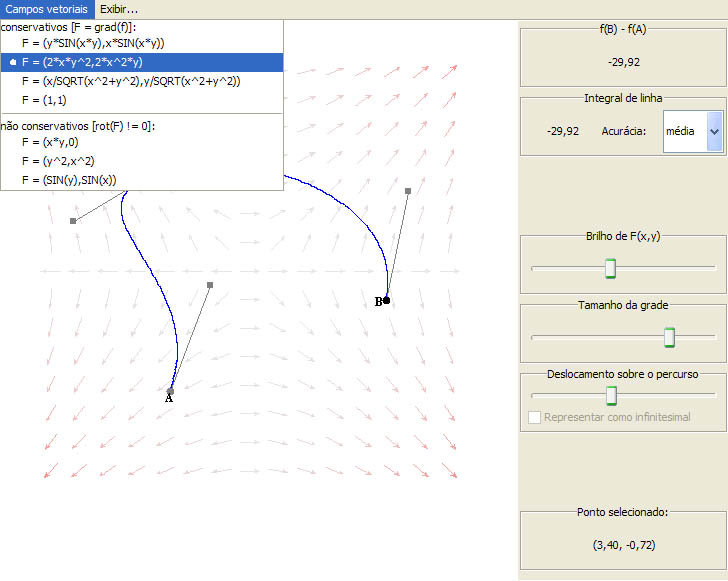
\includegraphics[width=\textwidth]{images/campo-vetorial.jpg}
			\caption{\footnotesize primeiro \foreign{applet} Java desenvolvido para o CEPA, em dezembro de 2007. Este recurso é expositivo, mas permite ao usuário interagir de modo a comparar seus cálculos com aqueles apresentados pelo \foreign{software}.}
			\label{fig:campo}
		\end{minipage}\hfill
		\begin{minipage}[b]{0.46\textwidth}
			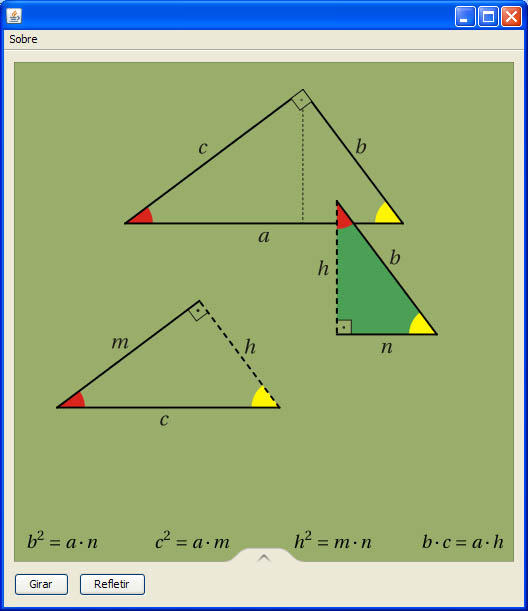
\includegraphics[width=\textwidth]{images/triangulo-retangulo.jpg}
			\caption{\footnotesize \foreign{software} desenvolvido para a proposta de aula interativa do CEPA, em maio de 2009. Este recurso é expositivo e colaborativo, pois foi feito para ser executado em lousas eletrônicas.}
			\label{fig:rel-metr}
		\end{minipage}
	\end{figure}
	
	A figura~\ref{fig:campo} ilustra o primeiro \foreign{applet} Java que desenvolvi quando ingressei no CEPA, em dezembro de 2007. Seu propósito é explorar os conceitos de integral de linha e de campos vetoriais conservativos ($\vec u = -\nabla f$) e não-conservativos. Essencialmente, o \foreign{software} exibe o valor da integral de linha, calculada numericamente.
	
	Inicialmente, o \foreign{software} disponibiliza um campo vetorial (conservativo) e um percurso fáceis de manipular, para que o usuário possa fazer os cálculos por conta própria, tanto da integral de linha quanto de $f(B) - f(A)$, oriundo do teorema fundamental do cálculo. Em seguida, ele é orientado a modificar o percurso, sem mover os pontos $A$ e $B$, e a perceber que a integral não muda (consequência do campo ser conservativo). Diferentemente, quando o usuário escolhe um campo não-conservativo, a integral altera-se com qualquer mudança no percurso. Este recurso está disponível \href{http://cepa.if.usp.br/old/files/simulation/javaapplet/PathIntegralAtContainer.html}{aqui}.
	
	A figura~\ref{fig:rel-metr} ilustra o aplicativo que foi desenvolvido especialmente para a proposta de aula interativa com lousa eletrônica do CEPA, para o projeto Aulas Interativas. Seu intuito é \emph{auxiliar o professor} a deduzir as relações métricas do triângulo-retângulo: o professor arrasta de dentro do triângulo maior (no topo) os dois triângulos-retângulos internos, e pode rotacioná-los e refletí-los convenientemente, de modo que fique evidente a relação de semelhança entre eles. Desta forma, o professor pode deduzir muito facilmente as relações, sem os embaraços da abordagem tradicional. Por exemplo, a relação $c^2 = a \cdot m$ pode ser deduzida observando-se os lados $a$ e $c$ do triângulo superior e os lados $c$ e $m$ daquele à esquerda: por semelhança, $c/m = a/c$, o que resulta na relação métrica.
	
	Pelo que observei nas apresentações desta aula, a simplicidade desta dedução foi o que realmente cativou os professores da Secretaria de Estado da Educação, e creio que tenha contribuido decisivamente para a participação do CEPA no projeto.
	
	\begin{figure}
		\centering
		\begin{minipage}[t]{0.46\textwidth}
			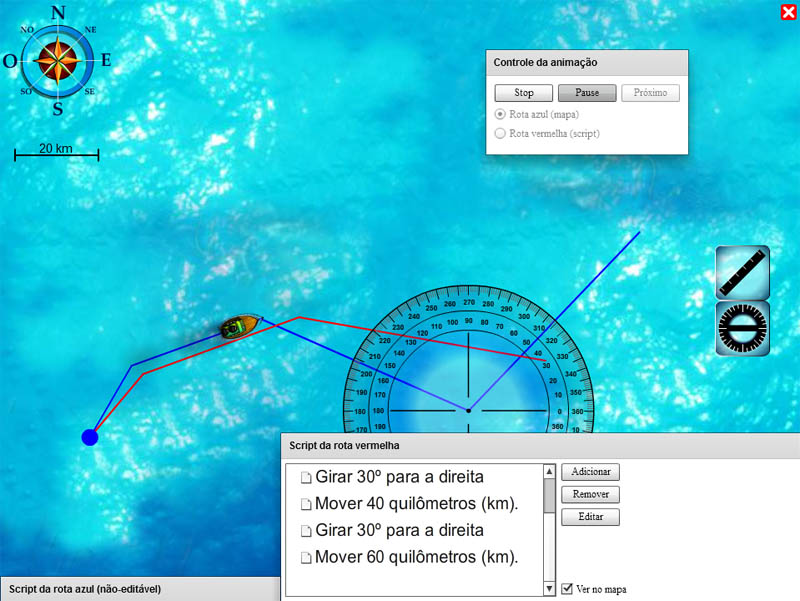
\includegraphics[width=\textwidth]{images/navigation.jpg}
			\caption{\footnotesize recurso desenvolvido para a disciplina de Matemática do 6\textordmasculine\ do Ensino Fundamental (projeto Aulas Interativas). Como o anterior, é expositivo e colaborativo, mas também permite avaliação do aluno, através da comparação entre os trajetos azul e vermelho.}
			\label{fig:nav}
		\end{minipage}\hfill
		\begin{minipage}[t]{0.46\textwidth}
			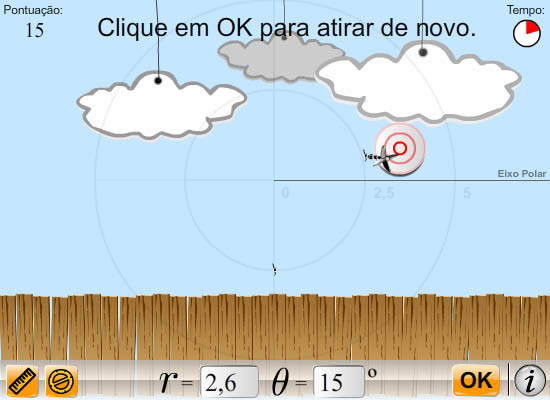
\includegraphics[width=\textwidth]{images/polar.jpg}
			\caption{\footnotesize este \foreign{software} foi desenvolvido para a Univesp, e traz uma abordagem mais próxima dos jogos eletrônicos. Ele também permite avaliação e foi feito para aulas a distância.}
			\label{fig:polar}
		\end{minipage}
	\end{figure}
	
	
	A figura~\ref{fig:nav} representa uma das atividades interativas que produzimos para o projeto Aulas Interativas, para a disciplina de Matemática do 6\textordmasculine\ ano do Ensino Fundamental. O intuito dela é permitir ao professor expor e exercitar, de maneira lúdica, conceitos como pontos cardeais, escala, medidas de ângulo e de distância, e até uma introdução à programação de computadores.
	
	Por exemplo, o professor pode desenhar uma trajetória (azul) arbitrária para o navio e, em seguida, pedir que os alunos representem aquela trajetória em termos de uma sequência de comandos \emph{mover}, \emph{girar} e \emph{repetir}. Isto também é feito no \foreign{software} (na lousa eletrônica), e é representado pelo script na base da imagem. Para executar esta tarefa a contento, os alunos devem utilizar a régua e o transferidor disponibilizados no \foreign{software}, bem como a escala do mapa. E para conferir a resposta, o professor pode habilitar a visualização desse caminho, em vermelho. Alternativamente, o professor pode escrever o script (rota em vermelho) e pedir que os alunos a desenhem, em azul. Observe ainda que o professor pode executar a animação do navio percorrendo a trajetória azul ou a vermelha passo-a-passo, e assim discutir cada instrução dada no script.
	
	Particularmente com relação a este \foreign{software}, outra possibilidade que chamou a atenção dos Professores Coordenadores das Oficinas Pedagógicas foi a possibilidade de ilustrar como é que o computador desenha uma curva: basta colocar uma instrução do tipo \emph{repetir 10 vezes os comandos: mover \unit{10}{\kilo\metre} e girar \unit{10}{\degree}}.
	
	Finalmente, a figura~\ref{fig:polar} ilustra outro recurso, este feito para a Univesp. Seu objetivo é permitir ao usuário \emph{familiarizar-se} com os sistema de coordenadas polar. Ao pressionar o botão \emph{ok} o alvo é aleatoriamente posicionado na tela, e cabe ao usuário acertá-lo com um dardo. Para lançar o dardo o usuário deve informar quais são as coordenadas, $r$ e $\theta$, do alvo. E quanto mais próximas da resposta, mais próximo do alvo o dardo chega e, por conseguinte, mais pontos ele faz. Há uma régua e um transferidor à disposição do usuário (embaixo, à esquerda), de modo que ele pode medir as coordenadas com precisão. No entanto, há um tempo limite para dar a resposta, e quanto mais rápido ele resolve a questão, mais pontos ele faz. Assim, para maximizar sua pontuação o usuário acaba concluindo, depois de algumas tentativas e erros, que é melhor \emph{estimar} a resposta. E deste modo espera-se que ele se familizarize com as coordenadas polares. Este recurso está disponível em \href{http://midia.atp.usp.br/atividades-interativas/AI-0001/}{aqui}.
	
	\section{Dados pessoais e produções relevantes}
\label{cap:resumo}
\small

%--------------------------------------------------------------------------
\subsection{Dados pessoais e de contato}
\addcontentsline{toc}{section}{Dados pessoais e de contato}

\begin{compactdesc}
  \item[Nome:] Ivan Ramos Pagnossin
  \item[RG:] 15.420.406-7
  \item[CPF:] 179.905.018-13
  \item[Celular:] +55 11 964.344.513
  \item[Telefone comercial:] (11) 3091-6695 ou 3091-6709
  \item[Endereço comercial:] CEPA (Centro de Ensino e Pesquisa Aplicada), Rua do Matão, Travessa R, 187
  Edifício Van de Graaf --- Cidade Universitária-USP --- São Paulo/SP --- CEP 05508-090
  \item[e-mail:] irpagnossin.edu@gmail.com ou irpagnossin@usp.br
  \item[Currículos:] \href{http://lattes.cnpq.br/6688104156301227}{Lattes} e \href{http://br.linkedin.com/in/irpagnossin}{LinkedIn} (veja a versão digital deste documento, disponível em \url{http://cepa.if.usp.br/ivan/memorial.pdf}).
\end{compactdesc}

%--------------------------------------------------------------------------
\subsection{Formação acadêmica e titulação}
\addcontentsline{toc}{section}{Formação acadêmica e titulação}

\begin{compactdesc}
  \item[Doutorado:] Doutor em Ciências, IFUSP (DFMT), 2005--2007.
  \item[Mestrado:] Mestre em Ciências, IFUSP (DFMT), 2002--2004.
  \item[Iniciação científica:] Laboratório de Física de Plasmas do IFUSP, 1997--1998.
  \item[Graduação:] Bacharel em Física Básica, IFUSP, 1997--2002.
  \item[Ensino Médio profissionalizante:] Técnico em eletrônica. Liceu de Artes e Ofícios de São Paulo, 1991--1995.
  \item[Ensino Médio:] Liceu de Artes e Ofícios de São Paulo, 1991--1995.
  \item[Ensino Fundamental:] Instituto São Pio X, 1982--1990.
\end{compactdesc}

%--------------------------------------------------------------------------
\subsection{Formação complementar}
\addcontentsline{toc}{section}{Formação complementar}

\begin{compactitem}
  \item \textsl{Capacitação SMART Board}, SMART, 22 de julho de 2011 (8 horas).
  \item \textsl{Leader Training II}, Arita Treinamentos, 2011 (35 horas).
  \item \textsl{Brigadista para combate ao incêndio}, Centro de Treinamento da Rochácara Ecofire, 2010 (12 horas).
  \item \textsl{Gerenciamento ágil de projetos com Scrum}, Caelum Ensino e Inovação, 2010 (20 horas).
  \item \textsl{Leader Training I}, Arita Treinamentos, 2010 (35 horas).
  \item \textsl{Desenvolvimento Web com HTML, CSS e JavaScript}, Caelum Ensino e Inovação, 2010 (20 horas).
  \item \textsl{Moodle na USP}, CEPA/CTI, 2008.
  \item \textsl{Francês}, Francês em casa, 2007 (50 horas).
  \item \textsl{Curso preparatório para o TOEFL}, Faculdade de Filosofia, Letras e Ciências Humanas da USP, 2006.
  \item \textsl{Curso de voo a vela}, Aeroclube Politécnico de Planadores, 2004--2009 (40 horas de voo).
  \item \textsl{Inglês}, Top English, 2002.
  \item \textsl{Alemão}, Faculdade de Filosofia, Letras e Ciências Humanas, 2003 (ouvinte do primeiro semestre do curso de Letras).
  \item \textsl{Cursinho para o exame vestibular}, Etapa, 1996.
  \item \textsl{Fundamentos de Astrofísica II --- Evolução estelar}, Escola Municipal de Astrofísica Planetário Municipal, 1993 (30 horas).
  \item \textsl{Tópicos de Astronomia: movimentos da Terra}, Escola Municipal de Astrofísica Planetário Municipal, 1993 (10 horas).
  \item \textsl{Reconhecimento do céu}, Escola Municipal de Astrofísica Planetário Municipal, 1992 (15 horas).
  \item \textsl{Desenho artístico}, Liceu de Artes e Ofícios de São Paulo, 1992.
  \item \textsl{Desenho técnico}, Liceu de Artes e Ofícios de São Paulo, 1991.
  \item \textsl{Cursinho para o exame vestibulinho}, Centro Educacional Desafio, 1990.
  \item \textsl{Curso Profissional de Datilografia}, Tecla Escola de Datilografia, 1989.
\end{compactitem}

%--------------------------------------------------------------------------
\subsection{Desenvolvimento de material didático ou instrucional}
\addcontentsline{toc}{section}{Desenvolvimento de material didático ou instrucional}

\begin{compactitem}
  \item 172 Objetos de Aprendizagem para \foreign{web} (Física e Matemática), no âmbito dos projetos Univesp e Redefor, sendo 32 produzidos por mim e 140 sob a minha coordenação.
  \item 104 Objetos de Aprendizagem para lousa eletrônica (Matemática e Língua Portuguesa), no âmbito do projeto Aulas Interativas, sendo 31 produzidos por mim e 73 sob a minha coordenação.
  \item 16 Objetos de Aprendizagem para \foreign{web} (Física), no âmbito do projeto TIDIA-Ae.
\end{compactitem}

%--------------------------------------------------------------------------
\subsection{Produção bibliográfica}
\addcontentsline{toc}{section}{Produção bibliográfica}

\begin{compactitem}

  \item Dissertações e teses
  \begin{compactitem}
    \item \textsl{Pontos-quânticos: fotodetectores, localização-fraca e estados de borda contra-rotativos}, Tese de Doutorado, IFUSP (2008).
    \item \textsl{Propriedades de transporte elétrico de gases bidimensionais de elétrons nas proximidades de pontos-quânticos de InAs}, Dissertação de Mestrado, IFUSP (2004).
  \end{compactitem}

  \item Artigos completos publicados em periódicos
  \begin{compactitem}
    \item I. R. Pagnossin, A. K. Meikap, T. E. Lamas, G. M. Gusev, J. C. Portal, \textsl{Anomalous dephasing scattering rate of two-dimensional electrons in double quantum well structures}, Phys. Rev. B, Condensed Matter and Materials Physics \textbf{78}, 115311 (2008). 
    \item I. R. Pagnossin, A. K. Meikap, A. A. Quivy, G. M. Gusev, \textsl{Electron dephasing scattering rate in two-dimensional GaAs/InGaAs heterostructures with embedded InAs quantum dots}, J. Appl. Phys. \textbf{104}, 073723 (2008).
    \item I. R. Pagnossin, E. C. F. da Silva, A. A. Quivy, S. Martini e C. S. Sergio, \textsl{The quantum mobility of a two-dimensional electron gas in selectively doped GaAs/InGaAs quantum wells with embedded quantum dots}, J. Appl. Phys. \textbf{97}, 113709 (2005).
  \end{compactitem}
		
  \item Trabalhos completos publicados em anais de congressos
  \begin{compactitem}
    \item R. S. Morais, V. C. R. Sarnighausen, I. R. Pagnossin, R. N. Marques, \textsl{O curso LC-EaD da USP: um olhar para o pólo Piracicaba no componente curricular Fundamentos de Matemática}, XVI Conferência GPIMEM: tecnologias digitais em Educação Matemática, Rio Claro (SP), Brasil (2013).
    \item I. R. Pagnossin, C. C. Cavalcanti, R. T. Soledade, G. da C. Marques, \textsl{Objetos de aprendizagem interativos: análise do desempenho dos alunos de ciências}, no II Congresso Internacional TIC e Educação (ticEduca), Lisboa, Portugal, 2012.
    \item I. R. Pagnossin, R. T. Soledade, C. C. Cavalcanti, \textsl{Atividades investigativas e colaborativas com objetos de aprendizagem interativos no curso semipresencial de Licenciatura em Ciências da USP/Univesp}, III Seminário Web Currículo PUC-SP, São Paulo (SP), Brasil (2012).
    \item I. R. Pagnossin, C. C. Cavalcanti, R. T. Soledade, G. da C. Marques, \textsl{Participação e desempenho de alunos no uso de objetos de aprendizagem interativos que simulam situações-problema na licenciatura em ciências da USP/Univesp}, I Simpósio Internacional de Educação a Distância e I Encontro de Pesquisadores em Educação a Distância, São Carlos (SP), Brasil (2012).    
    \item I. R. Pagnossin, G. M. Gusev, A. C. Seabra, A. A. Quivy, T. E. Lamas, J.-C. Portal, \textsl{Quantum Hall effect in bilayer system with array of antidots}, no 28th International Conference on the Physics of Semiconductors (ICPS-28), 2006, Viena. 28th International Conference on the Physics of Semiconductors (ICPS-28), 2006. p.~96.
    \item I. R. Pagnossin, G. M. Gusev, N. M. Sotomayor, A. C. Seabra, A. A. Quivy, T. E. Lamas, J.-C. Portal, \textsl{Quantum Hall effect in bilayer system with array of antidots}, no 28th International Conference on the Physics of Semiconductors (ICPS-28) --- Viena/Austria, 2006, Viena. Physics of Semiconductors, 28th International Conference, 2006. pp.~677 -- 678.
    \item I. R. Pagnossin, E. C. F. da Silva, A. A. Quivy, S. Martini, C. S. Sergio, \textsl{The influence of strain fields around InAs quantum dots on the transport properties of a two-dimensional electron gas confined in GaAs/InGaAs wells}, no 12th Brazilian Workshop on Semiconductor Physics, 2005, São José dos Campos. Brazilian Journal of Physics, 2005.
    \item I. R. Pagnossin, E. C. F. da Silva, A. A. Quivy, S. Martini, C. S. Sergio, \textsl{Scattering processes on a quasi-two-dimensional electron gas in GaAs/InGaAs selectively doped quantum wells with embedded quantum dots}, no 12th Brazilian Workshop on Semiconductor Physics, 2005, São José dos Campos. Brazilian Journal of Physics, 2005.
  \end{compactitem}
	
  \item Resumos publicados em anais de congressos
  \begin{compactitem}
    \item I. R. Pagnossin, E. C. F. da Silva, A. A. Quivy, J. R. Leite, S. Martini, C. S. Sergio, \textsl{The influence of an InAs layer on the quantum mobility of a two-dimensoinal electron gas in GaAs/InGaAs selectively doped quantum wells}, no XXVII Encontro Nacional da Matéria Condensada, 2004, Poços de Caldas. XXVII ENFMC, 2004. v. 1. pp.~399--399.
    \item I. R. Pagnossin, A. K. Meikap, A. A. Quivy, G. M. Gusev, \textsl{Weak localization and interaction effects in GaAs/InGaAs heterostructures with nearby InAs quantum-dots}, no 13th Brazilian Workshop on Semiconductor Physics --- São Paulo/SP, 2007, São Paulo. 13th Brazilian Workshop on Semiconductor Physics --- São Paulo/SP, 2007.
    \item I. R. Pagnossin, G. M. Gusev, A. C. Seabra, A. A. Quivy, T. E. Lamas, J.-C. Portal, \textsl{Quantum Hall effect in bilayer system with array of antidots}, no 28th International Conference on the Physics of Semiconductors (ICPS-28) --- Viena/Austria, 2006, Viena. 28th International Conference on the Physics of Semiconductors (ICPS-28) --- Viena/Austria, 2006.	
  \end{compactitem}
	
  \item Apresentações de trabalhos
  \begin{compactitem}
    \item R. S. Morais, V. C. R. Sarnighausen, I. R. Pagnossin, R. N. Marques, \textsl{O curso LC-EaD da USP: um olhar para o pólo Piracicaba no componente curricular Fundamentos de Matemática}, XVI Conferência GPIMEM: tecnologias digitais em Educação Matemática, Rio Claro (SP), Brasil (2013).    
    \item I. R. Pagnossin, C. C. Cavalcanti, R. T. Soledade, G. da C. Marques, \textsl{Participação e desempenho de alunos no uso de objetos de aprendizagem interativos que simulam situações-problema na licenciatura em ciências da USP/Univesp}, I Simpósio Internacional de Educação a Distância e I Encontro de Pesquisadores em Educação a Distância, São Carlos (SP), Brasil (2012).
    \item I. R. Pagnossin, M. H. Klein, P. P. L. Oliveira, \textsl{Inovação e Qualidade: Soluções Integradas na Produção de Materiais para EaD} (mesa redonda), 18\textordmasculine\ Congresso Internacional ABED de Educação a Distância, São Luís (MA), Brasil (2012).
    \item I. R. Pagnossin, G. da C. Marques, M. H. Klein, \textsl{Educação a distância na USP: da concepção à realização} (mesa redonda), 17\textordmasculine\ Congresso Internacional ABED de Educação a Distância, Manaus (AM), Brasil (2011).
    \item A. Yamin, H. dos Santos, I. R. Pagnossin, M. Alves, E. ter Haar, \textsl{Apoio técnico-pedagó\-gico aos projetos Redefor e à nova Licenciatura em Ciências na USP}, São Paulo (SP), Brasil (2011).
    \item I. R. Pagnossin, E. C. F. da Silva, A. A. Quivy, S. Martini, C. S. Sergio, \textsl{The influence of strain fields around InAs quantum dots on the transport properties of a two-dimensional electron gas confined in GaAs/InGaAs wells}, no 12th Brazilian Workshop on Semiconductor Physics, 2005, São José dos Campos. Brazilian Journal of Physics, 2005.
    \item I. R. Pagnossin, E. C. F. da Silva, A. A. Quivy, S. Martini, C. S. Sergio, \textsl{Scattering processes on a quasi-two-dimensional electron gas in GaAs/InGaAs selectively doped quantum wells with embedded quantum dots}, no 12th Brazilian Workshop on Semiconductor Physics, 2005, São José dos Campos. Brazilian Journal of Physics, 2005.
    \item XVIII Encontro Nacional de Física da Matéria Condensada. \textsl{The influence of strain fields around InAs quantum dots on the transport properties of a two-dimensional electron gas confined in GaAs/InGaAs wells}, Santos (SP), Brasil (2005).
    \item XVII Encontro Nacional de Física da Matéria Condensada, \textsl{A influência de pontos-quânticos de InAs sobre a mobilidade quântica de gases bidimensionais de elétrons confinados em poços-quânticos de GaAs/InGaAs seletivamente dopados}, Poços de Caldas (MG), Brasil (2004).
  \end{compactitem}
\end{compactitem}

%--------------------------------------------------------------------------
\subsection{Relatórios técnicos}
\addcontentsline{toc}{section}{Relatórios técnicos}

\begin{compactitem}
  \item 12 relatórios de atividade, para a FAPESP, referentes ao trabalho de desenvolvimento de \foreign{softwares} educacionais utilizando Java, no âmbito do projeto TIDIA-Ae, durante o período de dezembro de 2007 a janeiro de 2009. Esses relatórios podem ser obtidos através de \cite{irpagnossin-stoa}.
  \item 7 relatórios mensais de atividade, para o Instituto de Pesquisa Eldorado, referentes ao trabalho de produção de \foreign{softwares} educacionais para o projeto Aulas Interativas, durante o período de dezembro de 2009 a junho de 2010.
\end{compactitem}

%--------------------------------------------------------------------------
\subsection{Bolsas e auxílios}
\addcontentsline{toc}{section}{Bolsas e auxílios}

\begin{compactitem}
  \item Capacitação Técnica, nível TT-5, FUSP, 2010--2013.
  \item Capacitação Técnica, nível TT-4, FAPESP, 2008.
  \item Doutorado, FAPESP, 2005--2007.
  \item Mestrado, FAPESP, 2002--2004.
  \item Iniciação científica, CNPq, 1998.
  \item Iniciação científica, CNPq, 1997.
  \item Ensino Médio Profissionalizante, Liceu de Artes e Ofícios de São Paulo, 1991--1995.
\end{compactitem}

%--------------------------------------------------------------------------
\subsection{Auxílios para viagens ao exterior}
\addcontentsline{toc}{section}{Auxílios para viagens ao exterior}

\begin{compactitem}
  \item Grenoble High Magnetic Field Laboratory, Grenoble, França (março a maio de 2007). Estágio financiado pela FAPESP como parte do trabalho de doutorado.
\end{compactitem}

%--------------------------------------------------------------------------
\subsection{Participação em eventos}
\addcontentsline{toc}{section}{Participação em eventos}

\begin{compactitem}
  \item XVI Conferência GPIMEM, UNESP, Rio Claro (SP), Brasil (2013).
  \item 18\textordmasculine\ Congresso Internacional ABED de Educação a Distância (CIAED), São Luís (MA), Brasil (2012).
  \item I Simpósio Internacional de Educação a Distância e I Encontro de Pesquisadores em Educação a Distância (SIED:EnPED), São Carlos (SP), Brasil (2012).
  \item 17\textordmasculine\ Congresso Internacional ABED de Educação a Distância (CIAED), Manaus (AM), Brasil (2011).
  \item XVIII Encontro Nacional de Física da Matéria Condensada, Santos (SP), Brasil (2005).
  \item 12th Brazilian Workshop on Semiconductor Physics, São José dos Campos (SP), Brasil (2005).
  \item XVII Encontro Nacional de Física da Matéria Condensada, Poços de Caldas (MG), Brasil (2004).
\end{compactitem}

%--------------------------------------------------------------------------
\subsection{Organização de eventos}
\addcontentsline{toc}{section}{Organização de eventos}

\begin{compactitem}
  \item \LaTeX\ e a Internet, CEPA (2008).
\end{compactitem}

%--------------------------------------------------------------------------
\subsection{Projetos de pesquisa}
\addcontentsline{toc}{section}{Projetos de pesquisa}

\begin{compactitem}
  \item Estudo e desenvolvimento dos processos de criação e produção de Objetos de Aprendizagem para o projeto Univesp, junto à CTI e financiado pela FUSP (projeto Univesp), 2010.
\end{compactitem}

%--------------------------------------------------------------------------
\subsection{Cursos e treinamentos produzidos}
\addcontentsline{toc}{section}{Cursos e treinamentos produzidos}

\begin{compactitem}
  \item \textsl{Processo de Criação de Objetos de Aprendizagem: usos do Padrão SCORM}, disciplina do curso de pós-graduação a distância em design instrucional do Senac/SP, Brasil (2013). Carga-horária: 32 horas.
  \item \textsl{Criação de objetos de aprendizagem e utilização do padrão SCORM}. Oficina criada para o \textsl{III Colóquio Regional de EAD, Cultura e Produção de Subjetividade} da UNIFEI Itajubá (MG), Brasil (2013). Carga-horária: 4 horas.
  \item \textsl{Aula temática com lousa interativa}, produzida para a abertura oficial do projeto Aulas Interativas, na Secretaria de Estado da Educação, em 6 de novembro de 2009.
  \item \textsl{Usando \LaTeX; pensando \TeX}, curso semi-presencial criado para a Superintendência de Tecnologia da Informação da USP, Brasil (2008). Carga-horária: 24 horas.
\end{compactitem}

%--------------------------------------------------------------------------
\subsection{Cursos e treinamentos ministrados}
\addcontentsline{toc}{section}{Cursos e treinamentos ministrados}

\begin{compactitem}
  \item \textsl{Processo de Criação de Objetos de Aprendizagem: usos do Padrão SCORM}, disciplina do curso de pós-graduação a distância em design instrucional do Senac/SP (março de 2013).
  \item \textsl{Processo de Criação de Objetos de Aprendizagem: usos do Padrão SCORM}, disciplina do curso de pós-graduação a distância em design instrucional do Senac/SP (agosto de 2012).
  \item Treinamento de professores da rede pública de Hortolândia para a aula temática apresentada na abertura oficial do projeto Aulas Interativas, Diretoria de Ensino de Sumaré (3--5 de novembro de 2009).
  \item \textsl{Usando \LaTeX; pensando \TeX}, CEPA/CTI, 24 horas (2009).
  \item \textsl{Usando \LaTeX; pensando \TeX}, CEPA/CTI, 20 horas (2008).
  \item \textsl{Usando \LaTeX; pensando \TeX}, CEPA, 15 horas (2008).
\end{compactitem}

%--------------------------------------------------------------------------
\subsection{\foreign{Softwares} produzidos}
\addcontentsline{toc}{section}{\foreign{Softwares} produzidos}

\begin{compactitem}
  \item Script LabTalk para a obtenção das mobilidades quânticas das sub-bandas de gases bidimensionais de elétrons a partir de oscilações de magnetoresistência (efeito Shubnikov-de Haas).
\end{compactitem}

%--------------------------------------------------------------------------
\subsection{Palestras}
\addcontentsline{toc}{section}{Palestras}

\begin{compactitem}
  \item I. R. Pagnossin, \textsl{O futuro do design instrucional} (mesa redonda), I Jornada de Design Instrucional (JORDI), São Paulo (SP), 2012.
  \item \textsl{Um modelo de aula interativa com lousa eletrônica}, CEPA, 19 de maio de 2009 (apresentação da proposta do CEPA para o projeto Aulas Interativas, para membros da SEE e da Dell).
  \item \textsl{Um modelo de aula interativa com lousa eletrônica}, Diretoria de Ensino de Sumaré, julho de 2009 (apresentação do projeto Aulas Interativas para os diretores das escolas públicas de Hortolândia).
  \item \textsl{Tecnologia educacional: atividades interativas para EaD e lousas digitais}, CEPA, 23 de outubro de 2009 [apresentação feita para os alunos da disciplina FAP0459 (tecnologia educacional), a convite do Prof. Dr. Ewout ter Haar].
  \item \textsl{Atividades Interativas para EaD e lousas eletrônicas}, CTI, 13 de julho de 2010 (apresentação feita para os coordenadores do projeto Univesp, sobre uma proposta de atividades interativas para o mesmo projeto).
\end{compactitem}

%--------------------------------------------------------------------------
\subsection{Orientações e supervisões concluídas}
\addcontentsline{toc}{section}{Orientações e supervisões concluídas}

\begin{compactitem}
  \item Coordenação de uma equipe de 4--6 programadores para a produção de \foreign{softwares} educacionais para o projeto Aulas Interativas. De julho de 2009 a agosto de 2010.
  \item Coordenação de uma equipe de 6 programadores e 1 ilustrador para a produção de Objetos de Aprendizagem para os projetos Univesp e Redefor. De agosto de 2010 a dezembro de 2011.
\end{compactitem}

%--------------------------------------------------------------------------
\subsection{Orientações e supervisões em andamento}
\addcontentsline{toc}{section}{Orientações e supervisões em andamento}

\begin{compactitem}
  \item Coordenação de uma equipe de 1 programador e 1 ilustrador para a produção de Objetos de Aprendizagem para o projeto Univesp. Desde dezembro de 2011.
\end{compactitem}


	
	\begin{thebibliography}{+++}

	\bibitem{pagnossin-2005-1} I. R. Pagnossin, E. C. F. da Silva, A. A. Quivy, S. Martini e C. S. Sergio, \textsl{The quantum mobility of a two-dimensional electron gas in selectively doped GaAs/InGaAs quantum wells with embedded quantum dots}, J. Appl. Phys. \textbf{97}, 113709 (2005).
	
	\bibitem{pagnossin-2004-2} XVII Encontro Nacional de Física da Matéria Condensada, \textsl{A influência de pontos-quânticos de InAs sobre a mobilidade quântica de gases bidimensionais de elétrons confinados em poços-quânticos de GaAs/InGaAs seletivamente dopados}, 2004 (Poços de Caldas).
	
	\bibitem{pagnossin-2005-2} XVIII Encontro Nacional de Física da Matéria, \textsl{The influence of strain fields around InAs quantum-dots on the transport properties of a two-dimensional electron gas confined in GaAs/InGaAs wells}, 2005 (Santos);
	
	\bibitem{pagnossin-2005-3} 12th Brazilian Workshop on Semiconductor Physics, \textsl{The influence of strain fields around InAs quantum-dots on the transport properties of a two-dimensional electron gas confined in GaAs/InGaAs wells}, 2005 (São José dos Campos);
	
	\bibitem{pagnossin-2004-1} I. R. Pagnossin, \textsl{Propriedades de transporte elétrico de gases bidimensionais de elétrons nas proximidades de pontos-quânticos de InAs}, Dissertação de Mestrado, IFUSP, São Paulo (2004).
	
	\bibitem{silva-2003} M. J. da Silva, A. A. Quivy, S. Martini, T. E. Lamas, E. C. F. da Silva e J. R. Leite, \foreign{InAs/GaAs quantum dots optically active at \unit{1.5}{\micro\metre}}, Appl. Phys. Lett. \textbf{82}, 2646 (2003).
	
	\bibitem{johnson-1992} B. L. Johnson, C. Barnes, G. Kirczenow, \textsl{Theory of the Hall effect in two-dimensional quantum-dot arrays}, Phys. Rev. B \textbf{46}, 15302 (1992).
	
	\bibitem{pagnossin-2006} 28th International Conference on the Physics of Semiconductors, \textsl{Quantum Hall effect in bilayer system with array of antidots}, 2006 (Áustria).
	
	\bibitem{pagnossin-2008-1} I. R. Pagnossin, A. K. Meikap, A. A. Quivy, G. M. Gusev, \textsl{Electron dephasing scattering rate in two-dimensional GaAs/InGaAs heterostructures with embedded InAs quantum dots}, J. Appl. Phys. \textbf{104}, 073723 (2008).
	
	\bibitem{pagnossin-2008-2} I. R. Pagnossin, A. K. Meikap, T. E. Lamas, G. M. Gusev, J. C. Portal, \textsl{Anomalous dephasing scattering rate of two-dimensional electrons in double quantum well structures}, Phys. Rev. B, Condensed Matter and Materials Physics \textbf{78}, 115311 (2008). 
	
	\bibitem{pagnossin-2007} 13th Brazilian Workshop on Semiconductor Physics, \textsl{Weak localization and interaction effects in GaAs/InGaAs heteroestructures with nearby quantum-dots}, 2007 (São Paulo).
	
	\bibitem{tidia} TIDIA-Ae (Tecnologia da Informação no Desenvolvimento da Internet Avançada --- Aprendizado Eletrônico), em \url{http://tidia-ae.usp.br/portal}.
	
	\bibitem{applets} Alguns \foreign{applets} desenvolvidos na fase inicial do meu trabalho no CEPA: \url{http://goo.gl/yLLcg}, \url{http://goo.gl/LrdHn} e \url{http://goo.gl/s2igw}.
	
	\bibitem{irpagnossin-stoa} Relatórios sobre a utilização de Java e SVG como plataforma para o desenvolvimento de Objetos de Aprendizagem, em \url{stoa.usp.br/irpagnossin/files}, item ``Apresentação e relatórios técnicos''.
	
	\bibitem{curso-LaTeX} Curso \textsl{Usando \LaTeX; pensando \TeX}, em \url{http://goo.gl/bz6ST} (2011.06.15).
	
	\bibitem{mit} Cursos a distância do MIT (Massachusetts Institute of Technology), em \url{ocw.mit.edu} (2011.06.15).
	
	\bibitem{redefor} Rede São Paulo de Formação Docente, em \url{redefor.usp.br} (2011.06.15).
	
	\bibitem{aulas-interativas} Por exemplo, ``Lousas digitais ligadas à internet são usadas em escolas do interior de São Paulo'', em \url{http://goo.gl/T3dz0} (2011.06.15).
	
	\bibitem{ipad} Veja, por exemplo, \textsl{Escola brasileira substitui apostilas de papel por iPad}, em \url{http://goo.gl/eJ1pP}, \textsl{iPad: escola do Ceará vai utilizar o tablet como ferramenta de ensino}, em \url{http://goo.gl/2BlMK}, ou \textsl{New York orders thousands of iPads for schools}, em \url{http://goo.gl/Pkecg} (2011.06.15).
	
	\bibitem{melare-2009} Guia didático sobre as tecnologias da comunicação e informação, Daniela Melaré Vieira Barros, Vieira e Lent, Rio de Janeiro, 2009.
	
	\bibitem{homem-virtual} Projeto Homem Virtual, em \url{projetohomemvirtual.com.br} (2011.06.15).
	
	\bibitem{geogebra} Geogebra, \foreign{software} de geometria dinâmica, em \url{http://www.geogebra.org/cms/} (2011.06.15).
	
	\bibitem{igeom} iGeom, \foreign{software} de geometria dinâmica desenvolvido pelo Prof. Dr. Leônidas de Oliveira Brandão, do Instituto de Matemática e Estatística da USP, em \url{www.ime.usp.br/~leo/imatica/igeom} (2011.06.15).
		
	\bibitem{coelho-sabido} Coelho Sabido, \foreign{software} educativo para o ensino fundamental, em \url{coelhosabido.com.br} (2011.06.15).
	
	\bibitem{phet} Projeto PhET, em \url{phet.colorado.edu} (2011.06.15).
	
	\bibitem{lock-in} Amplificador \foreign{lock-in} virtual, da National Instruments, em \url{http://goo.gl/HBvKX} (2011.06.15).
	
	\bibitem{falstad} \foreign{Applets} Java para a visualização de conceitos de Física, Matemática e Engenharia, em \url{falstad.com} (2011.06.15).
	
	\bibitem{fendt} \foreign{Applets} Java de Física, traduzido pelo CEPA: \url{www.walter-fendt.de/ph14br} (2011.06.15).	
	
	\bibitem{merlot} Repositório de Objetos de Aprendizagem MERLOT, em \url{www.merlot.org/merlot} (2011.06.15).
	
	\bibitem{phet-research} Lista de artigos sobre as pesquisas acerca das simulações ciradas no projeto PhET\cite{phet}, em \url{phet.colorado.edu/en/research} (2011.06.15).
	
\end{thebibliography}	
	\addcontentsline{toc}{chapter}{Referências}

\end{document}
%-------------------------------------------------------------------------------
